%第3章


\section{感染症予防サポートシステムの概要}

本節では,感染症予防サポートシステムの目的,要求仕様及び概要を述べる.

% まず,スマートモビリティレジシステムの目的としては既存の無人レジ店舗のような複雑で高価なシステムではなく,小規模や中規模の企業でも導入できる安価なスマートモビリティレジシステムの作成である.この目的を基にし,スマートモビリティ決済システムは,下記の3点の要求事項を満たす必要がある.
まず,本システムにおいては,二酸化炭素濃度に加え,温度,湿度や人数といった環境値を観測,評価するシステムで以下の条件を満たすことを目的とした.
% \begin{itemize}
% \item 従来のセルフレジよりコストは抑えられる.
% \item 既存の中小店でも導入が容易.
% \item 従来のセルフレジより簡単な動作で決済まで行える.
% \end{itemize}
\begin{itemize}
    \item あらかじめ指定されたガイドラインだけでなく,部屋の特性にも配慮して評価を行える.
    \item 導入が容易でセンサデバイスを部屋の任意の場所に設置できる.
    \item 在室している人に対して感染リスク,および対処法を分かりやすく示すことができる.
    \item 入室しようとしている人に対しても部屋の滞在人数や感染リスクを分かりやすく示すことができる.
\end{itemize}
% 上述の「従来のレジよりコストは抑えられる.」という評価軸には,カゴ90台を導入するコストと,登録機1台1,875,000円と精算機$2,750,000円\times7台$として,合わせておよそ21,125,000円\cite{super}とレジの店員分の人件費を合わせたコストを比べた際,よりコストを抑えられるかということである.また,上述の「従来のレジより簡単な動作での決済まで行える.」という要求項目は,従来の店員のように,商品を手に取り,バーコードリーダで商品のバーコードを読み取り,カゴへ入れるという動作と全く同じ動作をしないということである.

以上のような目的を定めた理由を下記に述べる.
本システムは,学校の教室など,数人から数十人程度が使用する大きさの部屋を対象として考えた.
しかしながら,学校の教室を例にとってみても,同じ敷地面積であったとしても,設置されている場所によって,窓の数や部屋の形状は大きく異なり,同一の尺度で評価をするのは理想的とは言えない.
そこで,学校などの団体によって敷地面積に対しての適正収容人数や換気を行う時間間隔がガイドラインとして定められている場合であっても,そのガイドラインだけでなく,実際の環境値から予測される部屋の特性も考慮したうえで環境を評価する必要があるとした.
また,教室の中においても入り口付近と窓の近くによっては,換気状況などが変わってくる場合があり,それらも容易に観測できるよう,センサデバイスの専有面積を手のひら程度の小ささにし,場所の制約を少なくする必要があるとした.
そのほか,市販されているものの多くが,温湿度,二酸化炭素濃度で観測された値をそのまま表示しているものもとなっているが,一般的にユーザーが知りたいのは値そのものではなく,その結果がよいのか悪いのか,どうしなければならないのかということである.
%それと同時に,温湿度,二酸化炭素濃度の値の結果,換気が必要になったらその情報を伝えなければいけないのは部屋の中にいる人たちである.
この情報は在室している人に対して分かりやすく通知し,その状況を改善する行動に移してもらう必要がある.
そのため,在室している人に対しては感染リスクを伝えるとともに,改善する方法が分かりやすく示される必要があるとした.
また,入室しようと考えている人は,部屋の滞在人数やそれによる感染リスクをあらかじめ入室する前に確認できることが望ましい.
このように,在室している人に対しては,入室前にその部屋の状況を確認できることが大切であると考え,これらを実現させることを目的とした.

以上の要求事項を満たすために,電池のみで長時間動作するセンサデバイス,その値を適切に評価する処理デバイス,および部屋の内外に簡潔で分かりやすく感染リスクや対処法を示す表示デバイスから構成される感染症予防サポートシステムを提案する.

このシステムの対象環境の想定を以下に示す.
\begin{itemize}
    \item 数人から数十人程度が使用する大きさの部屋であること.
    \item 天井など,Webカメラを設置すると部屋の大部分が映るとともに,部屋の中にいるほとんどの人から確認できる,見晴らしの良い場所があること.
    \item 学校や団体などのガイドラインによって,部屋面積に応じた滞在上限人数が決まっていること.
    \item 窓や換気扇があり,換気が可能な部屋であること.
    \item 加湿器やエアコンの操作ができ,加湿や温度調整が可能な環境であること.
    \item 1日のうち,夜中の時間帯など,ほぼ使用されない時間が,12時間程度存在していること.
\end{itemize}

このシステムの使用イメージ図を図\ref{system_image}に示す.
\begin{figure}[htbp]
    \centering
    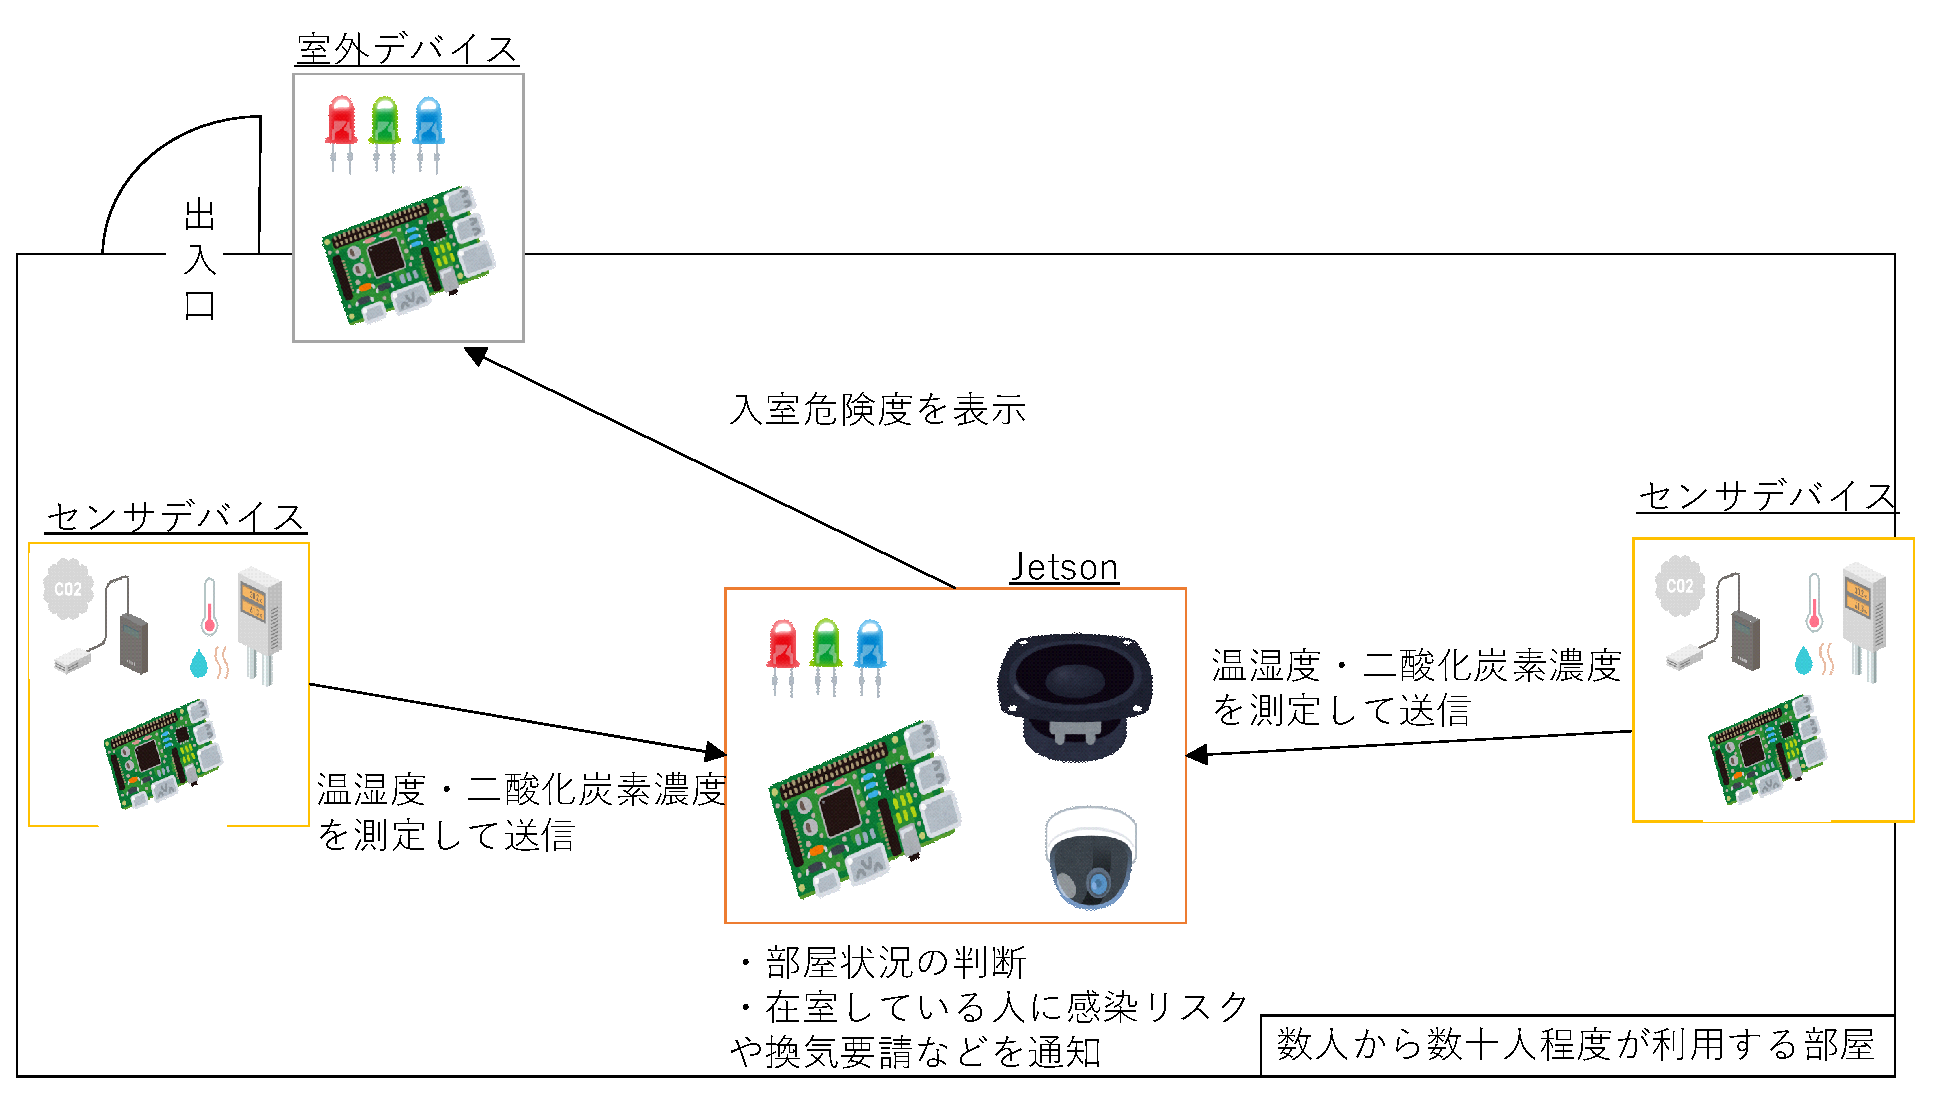
\includegraphics[width = 15cm]{./picture/system_image.eps}
    \caption{感染症予防サポートシステムの使用イメージ図}
    \label{system_image}
    \end{figure}

続いて,以下にこのシステムの動作の流れを述べる.
\begin{enumerate}
\item 部屋の複数箇所に設置されたセンサデバイスにより,各場所の温湿度,二酸化炭素濃度が測定される.
\item センサデバイスはその情報を処理デバイスであるJetsonに送信する.
\item 受信を行ったJetsonは受信した値と,接続されたWebカメラから得られた部屋の画像をもとに部屋の人数など,部屋状況の推定を行う.
\item 部屋状況をもとに,指定のガイドラインや部屋特性も把握したうえで現在の感染リスク,および換気が必要か否かを表示する.
\item 部屋の外にある表示デバイスに部屋の中の感染リスクを通知し,屋外デバイスはその内容を表示する.
\end{enumerate}

なお,本システムの開発は,Webカメラによる人数推定を伊藤大輝が,センサデバイスを稲田一輝が,屋外表示デバイスを小田恵吏奈が,処理デバイスを掛水誠矢が担当した.

% 以上の要求事項を満たすためには,本研究では,WebカメラとRaspberry Pi,各種センサを各買い物カゴに設置し,従来のセルフレジやセミセルフレジに比べて安価かつ簡単に決済できるスマートモビリティレジを提案する.

% 本研究において対象として設定したスーパーマーケットを下記の表\ref{taisho}に示す.


% \begin{table}[htb]
% \begin{center}
% \caption{対象スーパーマーケット}
% \begin{tabular}{|l|c|c|c|} \hline
% 店舗 & 売場面積(平方メートル) & レジ台数 & カゴ数 \\ \hline
% 小規模店舗,中規模店舗 & 1,200 & 7台 & 90個 \\ \hline
% \end{tabular}
% \label{taisho}
% \end{center}
% \end{table}


% 表\ref{taisho}を対象として設定した理由を下記に述べる.本研究では小規模店舗と中規模店舗のスーパーマーケットを対象とする.小規模店舗は「売場面積$800m^2未満」あるいは「売場面積800m^2~1,200m^2未満」の店舗,中規模店舗は「売場面積800m^2~1,200m^2未満」または「売場面積1,200m^2~1,600m^2未満」の店舗を指す\cite{super}.本研究では,小規模店舗と中規模店舗の平均である,売り場面積1,200m^2の店舗を本研究の対象の店舗とする.売場面積1,000m^2あたりレジ台数は,平均5.7台のため,対象の売場面積1,200m^2の店舗ではレジ台数平均6.84台と仮定できる\cite{super}.四捨五入でレジ台数は7台とし,それのレジ台数とする.また,売場面積が1,200m^2~1,600m^2$のスーパーマーケットの場合,平日レジ一台あたり一日客数は中央値として225.5人である\cite{super}.なお,平均営業時間は12.3時間のため,一時間あたり約18人の客がレジを使用すると予測できる\cite{super}.1人につき1個のカゴを使用しピーク時等の客入りを5倍,かつ店内に滞在する時間を1人につき1時間と仮定すると,約90個のカゴが必要と仮定した.


% 本研究で提案するシステムを使用する流れを図\ref{summary1}に示す.


% \begin{figure}[htbp]
% \centering
% \includegraphics[width = 15cm]{./picture/summary1.eps}
% \caption{商品識別システム全体の流れ}
% \label{summary1}
% \end{figure}



% まず,ユーザが買い物カゴを取って,顧客情報をカゴ情報と結び付ける.その後,顧客はカゴを持ち歩きながら商品を選んで,購入しようとした商品をカゴに入れる.その際,センシング技術を用いて,カゴ上に組み込まれた商品識別装置(カメラ等)による商品情報を取得しサーバへ情報を送信する.買い物を終える際は,カゴを返却するだけで決済が行われる流れとなる.本研究ではスマートモビリティレジシステム全体の流れについて設計を行ったが,最終的には,優先度が高い機能とした図\ref{summary1}に示す赤枠に囲まれる,カゴ上で商品情報を取得し決済を行う部分を開発対象とした.上記範囲のスマートモビリティレジシステムのイメージ図を以下の図\ref{summary2}に示す.


% \begin{figure}[htbp]
% \centering
% \includegraphics[width = 15cm]{./picture/summary2.eps}
% \caption{スマートモビリティレジシステムのイメージ図}
% \label{summary2}
% \end{figure}


% スマートモビリティレジシステムは識別・決済等を行うサーバ側,Raspberry PiとWebカメラ,および各種センサを設置した買い物カゴであるエッジ側(モビリティショッピング端末)の2つのパートで構成される.商品を各種センサが検知した際,Webカメラで商品のバーコードを撮影し,画像データ等をサーバへ送信する.サーバでは取得した商品のバーコード情報等を識別し,カゴに入れた商品の種類,金額,賞味期限,入れる時間などの情報を決済システムに一時的に保存し,仮登録する.ユーザはショッピングが終了する時点(例えば,決済ゲージを通る)に仮登録した商品の最終決済を行う.

% なお,本システムの開発は,サーバ側を段原丞治が,モビリティショッピング端末を真鍋樹が担当した.